\section{Validation}
In this section, we first describe how the system is tested and how we measure the quality of the code with SIG \cite{sig}. Afterwards we define a protocol with which the results of the system can be evaluated for correctness. We will first evaluate the results of the classification, and afterwards the relation scores. These are related in the sense that a relation score is calculated by the number of occurrences in labelled documents, so the correctness of labelling affects the correctness of relation scores.\\

\subsection{Testing the Application}
We will test the program using four different testing methods. The first is unit testing, which tests the separate components individually. Next comes integration testing, testing how well different components work together. Afterwards we use system testing for testing the different entire system. Last acceptance testing is used for testing how well the clients think the program works.

\subsubsection{Unit Tests}
Unit testing is done by writing automatic tests and making sure they pass every time the tests are executed. Unit tests test each method of a function separately, checking that the method does what it is supposed to do. If the method would need information from outside the class that information is mocked. This means that instead of using that other class, a fake object is made which returns a fake value. This ensures the tests will never fail due to changes in other classes.

\subsubsection{Integration Tests}
Integration testing uses automated tests which test how well different components of the system work together. This is done more or less the same as unit testing, however whilst you would mock methods from other classes in unit testing, with integration testing you do not. It is assumed that the separate modules are unit tested, therefor if an error occurs it is because something is wrong with the interaction between the modules and not with the modules themselves. 

\subsubsection{System Tests}
We are also planning to use system testing. System testing provides a more complete test of the entire system. This means it is useful to detect faults in the overall system, but less easy to determine where these faults may be located. System testing is done manually, which means the tests can not be easily repeated when the system changes whilst with other testing techniques this is possible.

\subsection{Acceptance Tests}
Last we use acceptance testing. This is testing done to see if the software does what the clients are expecting it to do. These tests are therefore also executed by the clients manually. Afterwards they can say what worked, what did not work, what was missing and what could be improved. For this, we set up an evaluation protocol.\\

\subsection{SIG}
SIG \cite{sig}, short for software improvement development group, is an organisation that analyses the code of projects to give insights in the quality of how the code is written. A high score means the code is highly maintainable and is kept simple. SIG includes Better Code Hub \cite{better_code_hub} which checks our code according to 10 guidelines as can be seen in appendix \ref{bch_guidelines}. The great thing about Better Code Hub is that it can be run at anytime. We can check Better Code Hub whenever, whilst for SIG we have to send in our code and wait for feedback.

\subsection{evaluating the classification}
There are several ways to evaluate machine learning algorithms. We will base our evaluation of the classifier on the guidelines of the Microsoft Azure Machine Learning evaluation model \cite{EvualteML}. According to the page binary classification can be evaluated with the following metrics: Accuracy, Precision, Recall, F1 and AUC.

\todo{eigen woorden:}

\subsubsection{Accuracy}
Accuracy is simply the proportion of correctly classified instances. accuracy doesn’t really capture the effectiveness of a classifier. In the income level classification scenario, assume you are testing on some data where 99\% of the instances represent people who earn less than or equal to 50K per year. It is possible to achieve a 0.99 accuracy by predicting the class “<=50K” for all instances. The classifier in this case appears to be doing a good job overall, but in reality, it fails to classify any of the high-income individuals (the 1\%) correctly.

\subsubsection{Confusion Matrix}
he class labels in the training set can take on only 2 possible values, which we usually refer to as positive or negative. The positive and negative instances that a classifier predicts correctly are called true positives (TP) and true negatives (TN), respectively. Similarly, the incorrectly classified instances are called false positives (FP) and false negatives (FN). \todo{matrix}

\begin{figure}[h]
\centering
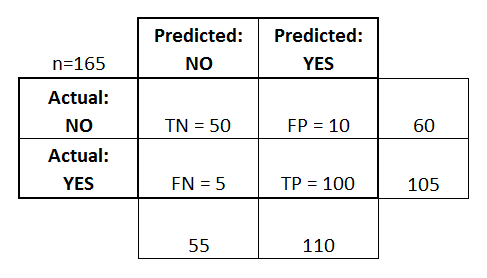
\includegraphics[width=0.5\textwidth]{confusion_matrix}
\caption{confusion matrix \protect\footnotemark{}}
\label{fig:confusion_matrix}
\end{figure}
\footnotetext{\url{https://docs.microsoft.com/en-us/azure/machine-learning/machine-learning-evaluate-model-performance}}


\subsubsection{Precision, Recall, F1 and UAC}
A very natural question is: ‘Out of the individuals whom the model predicted to be earning >50K (TP+FP), how many were classified correctly (TP)?’ This question can be answered by looking at the \textbf{Precision} of the model, which is the proportion of positives that are classified correctly: TP/(TP+FP). \\

Another common question is “Out of all the high earning employees with income >50k (TP+FN), how many did the classifier classify correctly (TP)”. This is actually the \textbf{Recall}, or the true positive rate: TP/(TP+FN) of the classifier. \\

Another related metric that is often used is the \textbf{F1} Score, which takes both precision and recall into consideration. It is the harmonic mean of these 2 metrics and is computed as such: F1 = 2 (precision x recall) / (precision + recall). \\

In addition, one can inspect the true positive rate vs. the false positive rate in the \textbf{Receiver Operating Characteristic (ROC) curve} and the corresponding \textbf{Area Under the Curve (AUC) value}. The closer this curve is to the upper left corner, the better the classifier’s performance is (that is maximizing the true positive rate while minimizing the false positive rate). Curves that are close to the diagonal of the plot, result from classifiers that tend to make predictions that are close to random guessing. \todo{graph}

\begin{figure}[h]
\centering
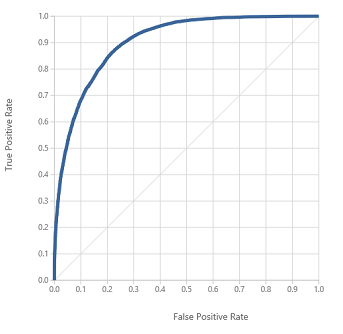
\includegraphics[width=0.5\textwidth]{UAC}
\caption{ROC / UAC graph \protect\footnotemark{}}
\label{fig:UAC}
\end{figure}
\footnotetext{\url{https://docs.microsoft.com/en-us/azure/machine-learning/machine-learning-evaluate-model-performance}}

\subsection{Evaluation of relation scores}
Evaluating relation scores is done differently. An important factor here is that cities have a natural relation due to their geographical position \cite{tobler1970computer}, so one would expect cities that lie close to each other are more related than cities that are on different sides of the country. This natural relation can be represented using the Gravity Model by Reilly \cite{reilly1931law}. The Gravity Model describes that the expected relation between two cities is based on the population of the two cities and the distance between these cities. A relation between two cities that is extracted from the data should thus expose a similar relative score as they would for the gravity model. Consider for example Amsterdam and Hoofddorp, which are cities that lie close to each other. Amsterdam is a large city, whereas Hoofddorp is much smaller. However, due to their close geographical position, the score that results from the Gravity Model would be high. If they turn out to have a very high score in our system, that would imply that the system is correct. Besides the Gravity Model, one can rely on the opinion of an expert in the field of urbanism that can judge whether an extracted relation is close to reality or not. We therefore agreed with the client that they would decide on a small set of relations whether they are correct. Lastly, the relations in the Randstad, a large urban area with the four largest cities of the Netherlands, have been examined before on the basis of firms \cite{van2010economic}. These relations can be compared to those extracted by the system.